
%(BEGIN_QUESTION)
% Copyright 2006, Tony R. Kuphaldt, released under the Creative Commons Attribution License (v 1.0)
% This means you may do almost anything with this work of mine, so long as you give me proper credit

Hobbyists building their own Tesla Coils often need to fabricate their own high-voltage capacitors for building the LC resonant circuit which is the heart of the coil:

$$\includegraphics[width=15.5cm]{i00317x01.eps}$$

One ingenious way to build such capacitors is to use old glass beer or soda bottles filled with salt water, with a metal rod or chain dipped into the water and aluminum foil wrapped tightly around the outside:

$$\includegraphics[width=15.5cm]{i00317x02.eps}$$

To obtain enough capacitance, one must usually group several of these beer-bottle capacitors together in parallel.  I mean, what's the point of having beer-bottle capacitors unless you can make a six-pack with them?

\vskip 10pt

As odd as it may seem, this actually has something to do with industrial instrumentation!  Identify which parts of the ``beer-bottle capacitor'' form the conductive plates of the capacitor and which part forms the dielectric.  Then identify how capacitance would be affected if we were to change the level of salt water in the beer bottle.  Finally, identify how this principle could be applied to the measurement of liquid level inside a vessel.

\vskip 20pt \vbox{\hrule \hbox{\strut \vrule{} {\bf Suggestions for Socratic discussion} \vrule} \hrule}

\begin{itemize}
\item{} Why use salt water instead of normal tap water?
\item{} If the bottle were made of thinner glass (all other factors being the same), would the capacitance {\it increase} or {\it decrease}?
\item{} If the bottle were taller (all other factors being the same), would the capacitance {\it increase} or {\it decrease}?
\item{} If the bottle were wider (all other factors being the same), would the capacitance {\it increase} or {\it decrease}?
\end{itemize}

\underbar{file i00317}
%(END_QUESTION)





%(BEGIN_ANSWER)

%(END_ANSWER)





%(BEGIN_NOTES)

The foil and water form the plates, while the glass forms the dielectric.  Capacitance increases as the salt water level increases.

\vskip 10pt

Capacitance formula:

$$C = {{A \epsilon} \over d}$$

\noindent
Where,

$C =$ Capacitance in Farads

$\epsilon =$ Permittivity of dielectric (absolute)

$A =$ Conductor area, in square meters

$d =$ Separation distance, in meters

\vskip 10pt

\begin{itemize}
\item{} Bottle made of thinner glass (all other factors being the same) -- capacitance will {\bf increase} (because $d$ becomes smaller)
\item{} Taller bottle (all other factors being the same) -- capacitance will {\bf increase} (because $A$ becomes larger)
\item{} Larger-diameter bottle (all other factors being the same) -- capacitance will {\bf increase} (because $A$ becomes larger)
\end{itemize}

%INDEX% Measurement, level: capacitance

%(END_NOTES)


